\documentclass[tikz, border=10pt]{standalone}
\usepackage{tikz}
\usetikzlibrary{positioning, fit, backgrounds, arrows.meta, calc}

\pgfdeclarelayer{containers}
\pgfsetlayers{containers,background,main}

\begin{document}
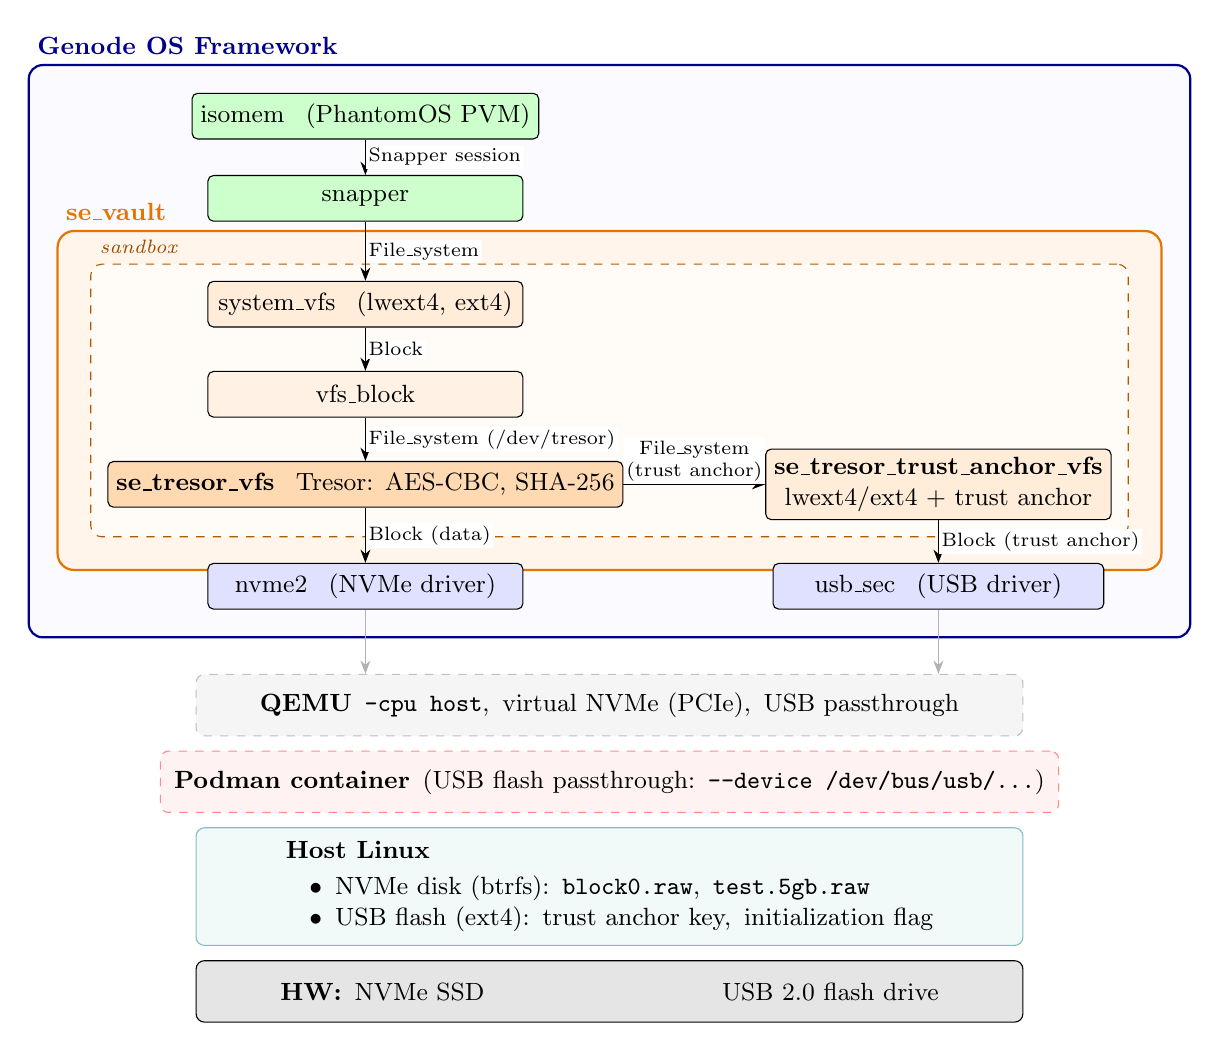
\begin{tikzpicture}[
  comp/.style={draw, rounded corners=2pt, align=center, font=\small,
               minimum width=4cm, minimum height=0.58cm, inner sep=3pt},
  rcomp/.style={draw, rounded corners=2pt, align=center, font=\small,
                minimum width=4.2cm, minimum height=0.58cm, inner sep=3pt},
  arr/.style={->, >=Stealth},
  note/.style={font=\scriptsize, fill=white, inner sep=1pt},
  band/.style={draw, rounded corners=3pt, align=left, font=\small,
               minimum width=10.5cm, minimum height=0.78cm, inner sep=5pt},
]

%% ---- Outside se_vault, inside Genode ----

\node[comp, fill=green!20] (isomem) {isomem \enspace (PhantomOS PVM)};

\node[comp, fill=green!20, below=0.45cm of isomem] (snapper) {snapper};

\draw[arr] (isomem) -- node[note, right]{Snapper session} (snapper);

%% ---- se_vault sandbox — left column (main data path) ----

\node[comp, fill=orange!15, below=0.75cm of snapper] (sysvfs)
    {system\_vfs \enspace (lwext4, ext4)};

\draw[arr] (snapper) -- node[note, right]{File\_system} (sysvfs);

\node[comp, fill=orange!10, below=0.55cm of sysvfs] (vfsblock)
    {vfs\_block};

\node[comp, fill=orange!30, below=0.55cm of vfsblock] (tresorvfs)
    {\textbf{se\_tresor\_vfs} \enspace Tresor: AES-CBC, SHA-256};

\draw[arr] (sysvfs)   -- node[note, right]{Block}                    (vfsblock);
\draw[arr] (vfsblock) -- node[note, right]{File\_system (/dev/tresor)} (tresorvfs);

%% ---- se_vault sandbox — right column (trust anchor) ----

\node[rcomp, fill=orange!15, right=1.8cm of tresorvfs] (ta_vfs)
    {\textbf{se\_tresor\_trust\_anchor\_vfs}\\lwext4/ext4 + trust anchor};

\draw[arr] (tresorvfs.east) --
    node[font=\scriptsize, fill=white, inner sep=1pt, align=center, above]
        {File\_system\\(trust anchor)}
    (ta_vfs.west);

%% ---- Block drivers (outside se_vault, inside Genode) ----

\node[comp,  fill=blue!12, below=0.7cm of tresorvfs] (nvme2)
    {nvme2 \enspace (NVMe driver)};

\node[rcomp, fill=blue!12] (usb_drv) at (ta_vfs |- nvme2)
    {usb\_sec \enspace (USB driver)};

\draw[arr] (tresorvfs.south) -- node[note, right]{Block (data)}         (nvme2.north);
\draw[arr] (ta_vfs.south)    -- node[note, right]{Block (trust anchor)}  (usb_drv.north);

%% ---- Containers (drawn back-to-front via layers) ----

%% se_vault outer box — on background (drawn first = below vault dashes)
\begin{pgfonlayer}{background}
\node[draw=orange!90!black, thick, rounded corners=6pt, fill=orange!8,
      inner sep=18pt,
      fit=(sysvfs)(vfsblock)(tresorvfs)(ta_vfs)] (sevault) {};

%% sandbox inner dashed box — on background (drawn second = on top of sevault)
\node[draw=orange!70!black, dashed, rounded corners=4pt, fill=orange!3,
      inner sep=6pt,
      fit=(sysvfs)(vfsblock)(tresorvfs)(ta_vfs)] (vault) {};
\end{pgfonlayer}

%% Labels for se_vault boxes
\node[font=\small\bfseries, text=orange!90!black, anchor=south west]
    at (sevault.north west) {se\_vault};
\node[font=\scriptsize\itshape, text=orange!60!black, anchor=south west]
    at (vault.north west) {sandbox};

%% Genode OS Framework box — on containers layer (bottommost)
\begin{pgfonlayer}{containers}
\node[draw=blue!55!black, thick, rounded corners=5pt, fill=blue!2,
      inner sep=10pt,
      fit=(isomem)(snapper)(sevault)(nvme2)(usb_drv)] (genode) {};
\end{pgfonlayer}
\node[font=\small\bfseries, text=blue!55!black, anchor=south west]
    at (genode.north west) {Genode OS Framework};

%% ---- Environment bands ----

\node[band, fill=gray!8, draw=gray!50, dashed,
      below=0.45cm of genode.south, anchor=north] (qemu)
    {\bfseries QEMU\normalfont\enspace
     \texttt{-cpu host},\enspace virtual NVMe (PCIe),\enspace USB passthrough};

\node[band, fill=red!5, draw=red!45, dashed,
      below=0.18cm of qemu.south, anchor=north] (podman)
    {\bfseries Podman container\normalfont\enspace
     (USB flash passthrough:\enspace\texttt{--device /dev/bus/usb/...})};

\node[band, fill=teal!5, draw=teal!50,
      below=0.18cm of podman.south, anchor=north] (hostl)
    {\bfseries Host Linux\normalfont\\[2pt]
     \hspace{0.3cm}$\bullet$\enspace NVMe disk (btrfs):\enspace
         \texttt{block0.raw},\enspace\texttt{test.5gb.raw}\\
     \hspace{0.3cm}$\bullet$\enspace USB flash (ext4):\enspace
         trust anchor key,\enspace initialization flag};

\node[band, fill=gray!20, draw=black,
      below=0.18cm of hostl.south, anchor=north] (hw)
    {\bfseries HW:\normalfont\enspace NVMe SSD \hspace{2.8cm} USB 2.0 flash drive};

%% ---- Arrows from block drivers through bands ----

\draw[->, >=Stealth, gray!60] (nvme2.south)   -- (nvme2.south   |- qemu.north);
\draw[->, >=Stealth, gray!60] (usb_drv.south) -- (usb_drv.south |- qemu.north);

\end{tikzpicture}
\end{document}
